\section{Layer~16 – Transcendence and Collective Cognition}
\label{sec:layer16}

% ----- SUPERKRACHT -----
\begin{tcolorbox}[colback=blue!5, colframe=blue!60, title=\textbf{Superpower: The Hive‑Mind}]
\begin{center}
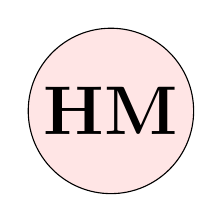
\begin{tikzpicture}
  \node[draw, circle, fill=red!10, minimum size=1.5cm, font=\bfseries\Huge] {HM};
\end{tikzpicture}
\textit{“What could we achieve together?”}
\end{center}
\end{tcolorbox}

One Pixel is clever, but \textbf{several Pixel‑like agents together}
are far cleverer.  Layer~16 lets them share knowledge, discuss, and
together arrive at better insights.

\begin{tcolorbox}[colback=yellow!5, colframe=yellow!80, title=Real‑life analogy]
A good study group can ace a difficult exam because everyone
understands a different piece of the material and explains it.
Layer~16 does the same, but lightning‑fast and over enormous
distances.
\end{tcolorbox}

\textbf{The swarm becomes a brain.}
Different Pixel robots can each explore a different part of the planet.
When they combine their discoveries, a total picture emerges that none
of them could have seen alone.  This transcends the sum of the parts –
a phenomenon scientists call \textbf{super‑additivity}.